%---------------------------------------
% PARTIE 2 : Organisation et déroulement
%---------------------------------------

\section{Déroulement et bilan technique}

\subsection{Planning prévisionnel}

\begin{figure}[H]
	\begin{center}
		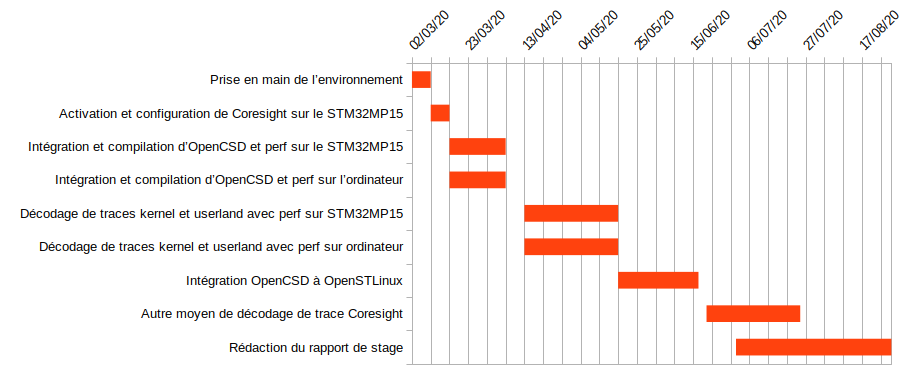
\includegraphics[width=\textwidth]{\pathPartTwo/gantt_previsionnel}
		\caption{Diagramme de Gantt du planning prévisionnel}
	    \label{fig:gantt_previsionnel}
	\end{center}
\end{figure}

\subsection{Planning effectif}

\begin{figure}[H]
	\begin{center}
		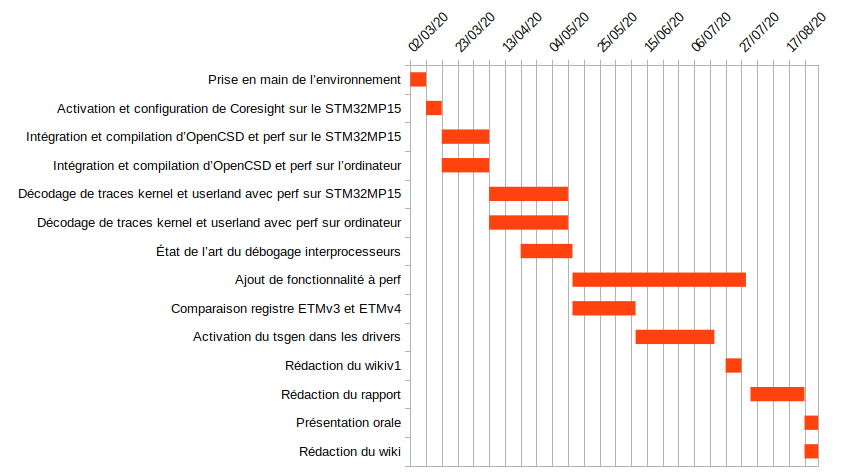
\includegraphics[width=\textwidth]{\pathPartTwo/gantt_effectif}
		\caption{Diagramme de Gantt du planning effectif}
	    \label{fig:gantt_effectif}
	\end{center}
\end{figure}

\subsection{Apport environnemental}
\label{sec:environmental_benefits}

En terme d'apport vis-à-vis de l'entreprise, plusieurs éléments auront été
légués à STMicroelectronics. Tout d'abord, même s'il n'y a pas eu de
document écrit concernant l'état de l'art du débogage interprocesseurs,
une réponse et une potentielle solution ont été données à l'oral lors de la
réunion organisée pour rendre compte de cette mission annexe. \\

De plus, le code source modifié sous forme de patchs a été envoyé sur le dépôt
GIT de l'entreprise. Une sauvegarde du code produit est disponible pour les
personnes souhaitant y accéder. Ce code, étant une solution temporaire à une
demande de l'entreprise, est par ailleurs en cours d'intégration au sein de la
branche ST du noyau Linux. Il comporte 7 fichiers et comptabilise 326 lignes
ajoutées et 27 retirées.  Le client, lors de l'utilisation de la distribution
fournie par ST, pourra ainsi utiliser le système Coresight puisqu'il sera
activé spécifiquement sur les cartes STM32MP15. Cela permettra par ailleurs de
déboguer les applications et programmes conçus au sein de l'espace noyau. \\

Enfin, la documentation des composants et du framework réalisée sur le Wiki
permet aux différents utilisateurs et aux clients une publication des
connaissances accumulées pendant le stage ainsi que la possibilité de
comprendre comment ce système fonctionne.

\subsection{Critique objective}
\label{sec:perf_criticism}

\subsubsection{perf}

Au vu du planning prévisionnel, la possibilité du développement d'un driver
Linux n'avait pas été prise en compte. Dans le planning effectif, le projet
s'est développé en cinq étapes : La prise en main et activation du
sous-système Coresight, l'intégration et le décodage de traces, l'état de
l'art du débogage interprocesseurs et enfin l'ajout de la fonctionnalité au
sein de perf. \\

Ayant eu auparavant une expérience avec la STM32MP1 lors d'un précédent
projet, la prise en main et l'activation de l'environnement ont été très
rapide.  De même, la mise en place du décodage des traces Coresight a été
rapide. C'est lors de cette étape d'ailleurs, où les crashs de perf des traces
du noyau Linux suivant les cas d'utilisation on été repérées. Et par la
suite, une initiative pour tenter de résoudre le problème a été pensée. \\

L'upstream à la communauté Linux n'est pour l'instant pas possible dans la
mesure où le travail accompli ne remplit pas les critères. Néanmoins, une
intégration au sein de la branche interne ST du noyau Linux peut être réalisé.
Un certain retard dans les opérations a engendré une multiplication des tâches
en parallèle. \\

Les deux derniers mois étaient destinés à la rédaction du rapport et les
taches annexes d'intégration du travail effectué. Une erreur lors des étapes
de validation et les retards cumulés ont entraînés une précipitation de la
rédaction du rapport au détriment de l'intégration du travail. De plus, une
erreur dans la validation a entraîné une impossibilité de réaliser certains
cas d'utilisation dans le but d'une démonstration. L'exposition par mail de ce
problème avec la liste de diffusion Coresight a permis une première
appréhension malgré le temps restant. \\

\subsubsection{État de l'art}
\label{sec:state_of_the_art}

Pour l'état de l'art, la compréhension et la mise en place d'un tel système
ont été plutôt longues à cause de la situation liée au Covid. Enfin lorsque le
plan d'action a été modifié pour la résolution du problème de crashs, la
majorité des difficultés problèmes est survenue. Il a fallu tout d'abord
étudier les registres des ETMs, et à ce moment, un retard dans les travaux
s'est accumulé. \\

À l'issue de cette mission annexe, un point particulier a été le manque
d'initiative pour créer un rapport sur cet état de l'art. Une réunion avec les
principaux acteurs de ce stage a été organisée pour exposer oralement les
différentes possibilités impliquées pour la mise en place d'une solution.
Néanmoins, et même s'il n'avait pas été demandé, un rapport écrit de la
situation avec une planification détaillée aurait été appréciable pour une
passation des savoirs et des travaux effectués. \\

Malgré tout, cela laisse entrevoir la possibilité du développement d'une
solution pour déboguer l'ensemble des trois coeurs du SoC par le biais d'une
seule application de l'espace utilisateur dans un éventuel futur projet.

%° Planning prévisionnel :

%- Prise en main de la plateforme STM32MP1 (une semaine) : DONE
%- Configurer/Activer Coresight sur la Plateforme (une semaine) : DONE
%- Intégrer OpenCSD dans perf sur le platforme (un mois) : DONE
%- Intégrer OpenCSD off target pour décodage sur host (un mois, fait en
%parallèle) : DONE
%- Décodage de traces kernel space et userland avec perf sur target (un mois)
%: STARTED
%- Décodage de traces kernal space et userland avec perf sur host (un mois en
%parallèle) : STARTED
%- Intégrer OpenCSD à Yocto (un mois)
%- Autre moyen de décoder et utiliser Coresight ? (2 mois en parallèle) :
%STARTED
%- Écriture du wiki (wiki.st.com) concernant Coresight (une semaine, deadline
%début Juin 2020)
%- Écriture du rapport de stage (2 mois, 2,5 mois en parallèle)
